\section{Paul Traps}
It's safe to say that Paul traps have proven their worth as a valuable tool for working with trapped ions. Even outside of quantum computing, experiments involving trapped ions have provided crucial insight to many fields of physics over the last few decades. For us in particular, Paul traps utilizing RF electric fields and stationary qubit arrays are the focus of much research involving 2D Coulomb crystals. Given that importance, we'll take this opportunity to examine the theory behind Paul traps and how they may be implemented experimentally.

\subsection{Theoretical Framework}
Studying the work of Leibfried \textit{et al.}, we see a common model used to describe the electric potential $\Phi(x, y, z, t)$ of an RF trap \cite{Leibfried}. This assumes a quadrupolar electrode layout, also known as point traps \cite{Bruzewicz}, and that the function for the potential can be decomposed into a time-independent (static) part and a time-dependent part that depends on the RF drive frequency $\omega_{RF}$ such that
\begin{align}
    \Phi(x, y, z, t) &= U \frac{1}{2}(\alpha x^2 + \beta y^2 + \gamma z^2)\\ 
    \nonumber&+ {\widetilde{U}} cos(\omega_{RF}t) \frac{1}{2}(\alpha' x^2 + \beta' x^2 + \gamma' z^2).
\end{align}
Taking into consideration that this potential needs to satisfy Laplace's equation at all times, we get conditions for the geometric factors
\begin{align}
    &\alpha + \beta + \gamma = 0\\
    \nonumber &\alpha' + \beta' + \gamma' = 0.
\end{align}
There are multiple choices of appropriate values here that define various confining fields. Of interest to us is the choice
\begin{align}
    -(\alpha + \beta) &= \gamma > 0\\
    \nonumber \alpha' &= -\beta'
\end{align}
which dynamically confines particles in the $x$-$y$ plane and, at the same time, statically confines postively charged particles in the $z$-direction.

Ultimately, the interaction of ions and electromagnetic fields is quantum mechanical in nature (the motion of the trapped ions is quantized and closely approximated by static potential harmonic oscillators). However, a classical formulation can provide a decent approximation in many settings \cite{Leibfried}.
\subsubsection{Classical Equations of Motion}
For simplicity, we'll consider motion only in the $x$-direction, but these equations are readily applied to motion in other directions. Using the potential in eq. (4), the motion of a particle with mass $m$ and charge $Z\abs{e}$ is given by
\begin{align}
    \ddot{x} &= -\frac{Z\abs{e}}{m} \partialderivative{\Phi}{x}\\
    \nonumber&= -\frac{Z\abs{e}}{m} \left[ U\alpha + \widetilde{U} \cos(\omega_{RF} t \alpha')\right] x
\end{align}
Using the substitutions
\begin{equation}
    \xi = \frac{\omega_{RF} t}{2}, \quad a_x = \frac{4Z\abs{e} U\alpha}{m \omega_{RF}^2}, \quad q_x = \frac{2 Z\abs{e} \widetilde{U}\alpha'}{m \omega_{RF}^2}
\end{equation}
we can rewrite Eq. (7) in the form of the Mathieu equation
\begin{equation}
    \derivative{^2 x}{\xi^2} + [a_x - 2q_x \cos(2\xi)] x = 0
\end{equation}
which is a known differential equation with periodic coefficients and having stable solutions that can be found with the Floquet theorem \cite{Leibfried}. 

For the sake of brevity, I'll leave out the complete derivation, but it suffices to say that the coefficients are recursively defined, and a numerical value must be extracted by truncating the continued fractions at the desired level of accuracy. The higher order contributions in the continued fraction typically fall off quickly for values of $a_x, q_x \ll 1$ in our region of interest \cite{Leibfried}.

What that work has done is allowed us to describe a region of stability in the potential field, and in particular, a lowest stability region---one which contains the point $(a_i, q_i) = (0,0), \quad \forall \: i \in \{x, y, z\}$. The actual shape of the stability region still depends on the geometric factors $\alpha$, $\beta$, and $\gamma$ which themselves depend on the applied RF field and trap electrodes. Looking at Fig. \ref{fig:Stability Region}(a) we see the lowest stability region of a Paul trap. $\beta_i$ represent the borderlines of stability, and in the case of the cylindrically symmetric Paul trap, $\beta_x = \beta_y$. A similar situation occurs for the linear trap which has borderlines of stability mirrored over the $q_x$ axis (Fig. \ref{fig:Stability Region}(b)).
\begin{figure}[h]
    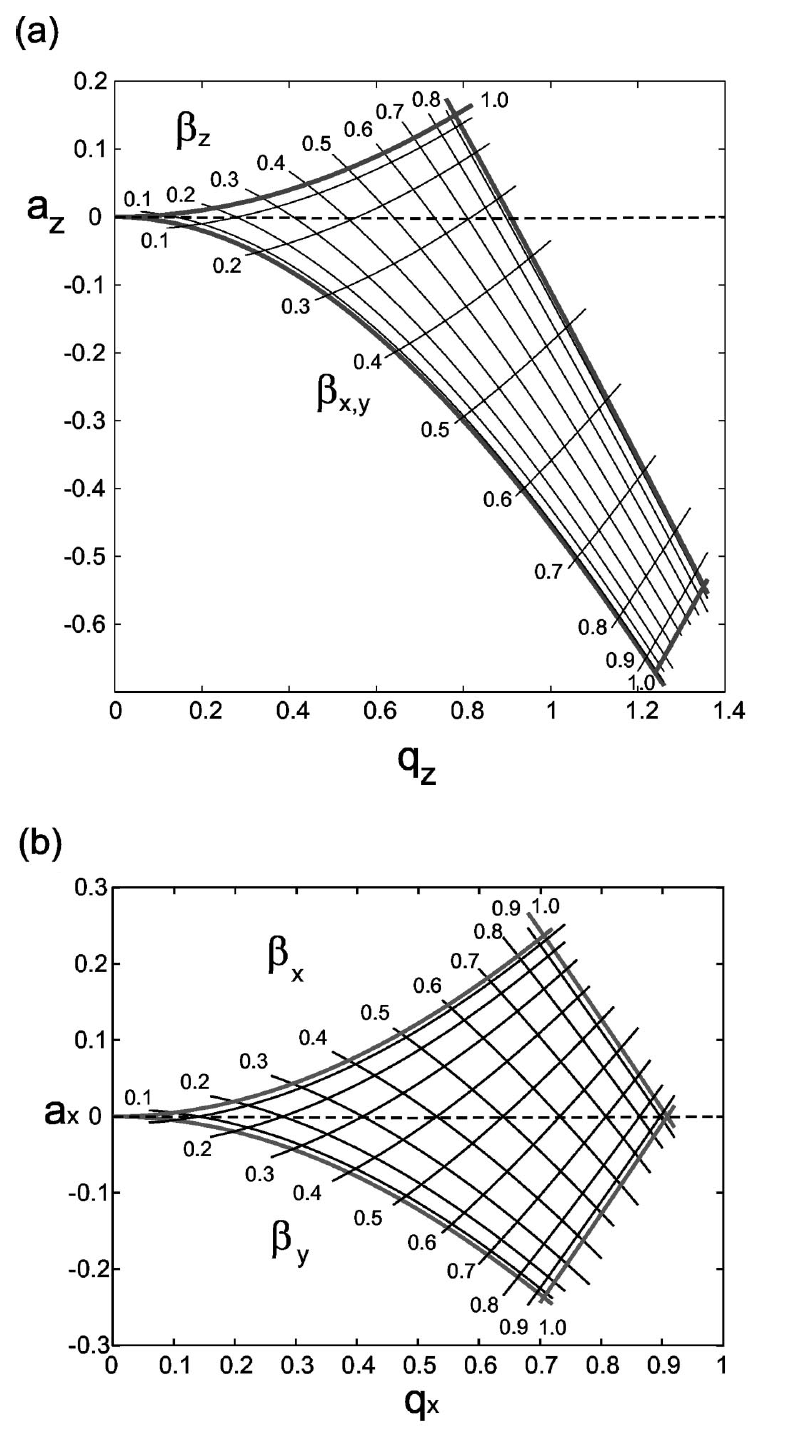
\includegraphics[width=\linewidth]{Leibfried - Stability Region.png}
    \caption{(\textbf{a}) Stability diagram for a cylindrically symmetric RF trap. This is the case that $\alpha=\beta = -\gamma/2$ and $\alpha'=\beta' = -\gamma'/2$. Confinement is observed in all three axes. (\textbf{b}) For comparison, this is a stability diagram for a linear trap with $\alpha+\beta = -\gamma$, $\alpha' = -\beta'$, and $\gamma'=0$. Figure borrowed and slightly modified from \textit{Quantum dynamics of single trapped ions} \cite{Leibfried}. Description is my own.}
    \label{fig:Stability Region}
\end{figure}
In general, however, it's not imperative that RF traps have an intrinsic symmetry and the borderlines of stability in those cases may not have such simple relationships \cite{Leibfried}.

We can now approximate the motion of an ion in such a quadrupole potential. In the manner of Brownnutt \textit{et al.} we get
\begin{equation}
    x(t) = X_0 \cos(\omega_t t + \varphi_0) \left[ 1 + \frac{q_x}{2} \cos(\omega_{RF} t) \right]
\end{equation}
where $\varphi_0$ is simply a phase that comes from initial conditions. Of more importance is $\omega_t$ and $\omega_{RF}$ which correspond to the "secular" motion and "micromotion" respectively. The secular, or trap, frequency $\omega_t$ is given by $\omega_t \approx \omega_{RF}/2$ and has a rather large amplitude that accounts for the bulk of the ion motion. The smaller motion, or micromotion, has a much smaller amplitude of $q_x/2$ that of the secular motion and oscillates at the drive frequency $\omega_{RF}$ \cite{Brownnutt}.

To give us an idea of some typical numbers, in a trap with a potential $V \sim \SI{500}{\volt}$ and ion-electrode spacing $d = \SI{500}{\micro\meter}$, we'd expect to see $\omega_{RF} \sim 2\pi \times \SI{20}{\mega\hertz}$ and $\omega_t \sim 2\pi \times \SI{2}{\mega\hertz}$ \cite{Brownnutt}.

This micromotion, as we've mentioned before, is detrimental to the successful operation of a quantum computer. Hence, it's of much importance to understand the entire picture when looking at motion of trapped ions.
\subsubsection{Quantum Mechanical Equations of Motion}
A more complete description of the motion of ions in an RF trap will require a quantum mechanical approach. We again follow in the footsteps of Leibfried \textit{et al.} and begin by writing the time-dependent potential $V(t)$ as
\begin{equation}
    V(t) = \frac{m}{2} W(t) \hat{x}^2
\end{equation}
where $W(t)$ is treated like a time-varying spring constant and is given by
\begin{equation}
    W(t) = \frac{\omega_{RF}^2}{4} [a_x + 2q_x \cos(\omega_RF t)].
\end{equation}
Using those equations, we can write the Hamiltonian of the motion, $\hat{H}^{(m)}$, which looks very similar to a static potential harmonic oscillator
\begin{equation}
    \hat{H}^{(m)} = \frac{\hat{p}^2}{2m} + \frac{m}{2} W(t) \hat{x}^2.
\end{equation}
Working directly off of Eq. (13) we get
\begin{align}
    \dot{\hat{x}} &= \frac{1}{i\hbar} [\hat{x}, \hat{H}^{(m)}] = \frac{\hat{p}}{m}\\
    \dot{\hat{p}} &= \frac{1}{i\hbar} [\hat{p}, \hat{H}^{(m)}] = -m W(t) \hat{x}
\end{align}
which leads to
\begin{equation}
    \ddot{\hat{x}} + W(t) \hat{x} = 0
\end{equation}
This is very similar to the Mathieu equation we found in Eq. (9). Enough so, that we can replace the operator $\hat{x}$ with a function $u(t)$ and it becomes possible to find solutions to Eq. (16) from the special solutions to the Mathieu equation with boundary conditions
\begin{equation}
    u(0) = 1, \quad \dot{u}(0) = i\nu.
\end{equation}
As before, I'll gloss over much of the derivation (leaving the reader free to explore \textit{Quantum dynamics of single trapped ions} for themselves) \cite{Leibfried} and arrive at the solution
\begin{equation}
    \braket{x'}{n, t} = \exp \left[ -i \left(n + \frac{1}{2} \right) \nu t \right] \chi_n (t)    
\end{equation}
where $\ket{n, t}$ are a set of basis states for $n = 1, 2, ..., \infty$ and $\chi_n(t)$ is a complex function that includes, amongst other things, the classical micromotion term appearing as a pulsation in the wave function with the same period as the RF driving field.

\subsection{Experimental Framework}
Now that we've examined some of the theory behind the trapping potentials and the motion of trapped ions, we can take a closer look at some experimental setups involving 2D crystals of ions and Paul traps. 
\subsubsection{Basic Structure}
The quadrupolar electrode layouts that we've discussed so far, also known as point traps, can be achieved in multiple ways as shown in Fig. \ref{fig:Paul traps}.
\begin{figure*}[t]
    \centering
    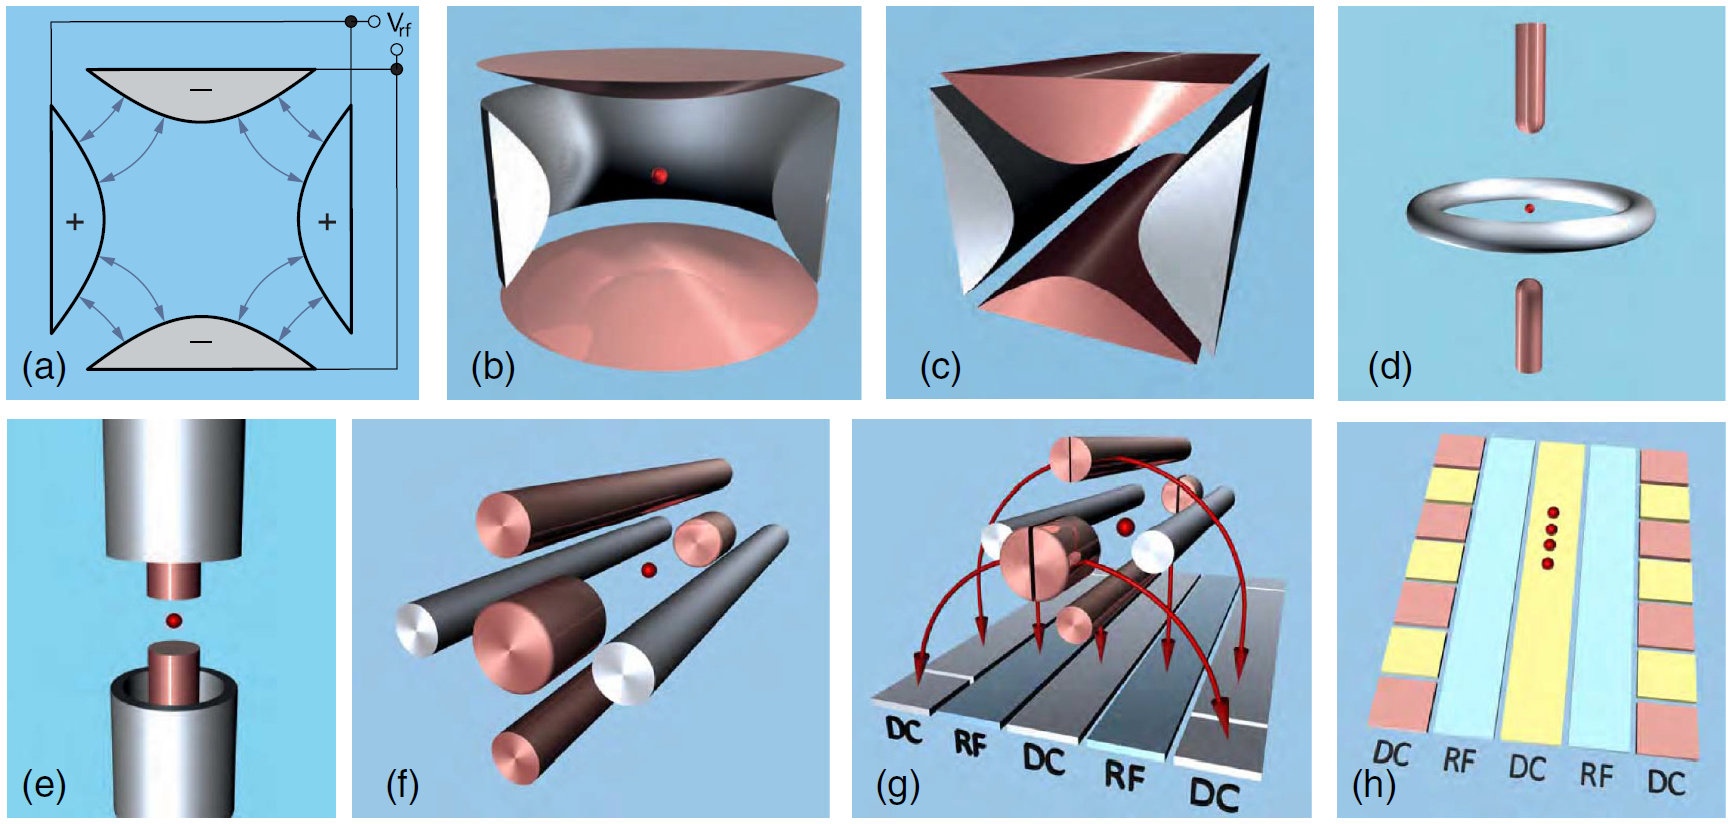
\includegraphics[width=\textwidth]{Brownnutt - Paul Traps.png}
    \caption{Several possible trap configurations are seen here. (\textbf{a}) In the simplist case, a set of four perfectly hyperbolic electrodes create a perfectly quadrupolar field. (\textbf{b}) This is a basic ring trap. It has rotational symmetry and an create a pseudopotential capable of confining ions in three dimensions. (\textbf{c}) This is translationally symmetric and forms the basis for a linear trap. (\textbf{d}), (\textbf{e}) These are both topologically equivalent to the ring trap in (b). (\textbf{f}) This is topologically equivalent to the linear trap in (c) but with additional endcap electrodes making it a four-rod linear trap. (\textbf{g}) The four-rod trap in (f) can be reconstructed so that the electrodes are flattened into a single plane. This forms a linear "surface-electrode" trap. (\textbf{h}) A linear trap similar to (g) except the electrodes have been segmented to allow for multiple trapping zones. Figure borrowed from \textit{Ion-trap measurements of electric-field noise near surfaces} \cite{Brownnutt}. Description is my own.}
    \label{fig:Paul traps}
\end{figure*}

Of greatest interest to our study of 2D Coulomb crystals are the surface, or planar, traps like those in Fig. \ref{fig:Paul traps}(g). Planar traps of this variety create a pseudopotential minimum above the surface where ions can be held at distances of $\sim \SI{100}{\micro\meter}$ from the electrode. By placing the electrodes in a single plane, we get the benefit of being able to build them on chips, which would be an advantage for a scalable quantum computer. Even more useful still are the segmented traps seen in Fig. \ref{fig:Paul traps}(h). With a point trap, it's not possible to place more than one ion at a point without increasing the undesirable micromotion. On the other hand, a segmented trap has separate, individually controlled segments allows for a single trap structure to contain multiple areas of potential minima that can hold an array of ions \cite{Brownnutt, Bruzewicz}. 

These are only the most basic trapping configurations. In reality, because fields from stray charges or imperfect fabrication can result in excess micromotion, traps will often require additional compensation electrodes to minimize those effects. For most practical purposes, these are ignored when analyzing trap behavior, but quickly considered if analyzing noise in the system \cite{Brownnutt}.

\subsubsection{Monolithic Traps}
Keeping the focus on surface traps for confining 2D Coulomb crystals, we'll take a look at some research involving monolithic traps. Monolithic traps are those where the components are integrated into a single piece, such as a microfabricated chip. Monolithic integration is expected to work in hand with modular approaches to manufacturing quantum technology. By combining chip-integrated components with a modular hierarchy, the hope is to realize scalability of quantum computers in a similar way to classical computers \cite{Bruzewicz}.

One such monolithic trap was implemented by Wang \textit{et al.} in 2020 to demonstrate confinement of over 20 \ion{171}{Yb}{+} ions in a stationary 2D ion crystal \cite{YeWang}. Their monolithic trap is constructed from a single plate of alumina (Al\textsubscript{2}O\textsubscript{3}) coated in gold. The trap consists of 20 electrodes, of which 14 are connected to ground with the remaining electrodes connected to DC sources. What makes their setup unique is that the structure of the electrodes allows for precise control over the orientation of the 2D crystal plane. This makes it possible to rotate the principle axes of the trap potential, keeping the micromotions constrained to the 2D plane and perpendicular to the Raman laser beams. This has a significant impact on reducing the effect of micromotion on coherent quantum operations \cite{YeWang}.

More recently, in 2023, work by Kiesenhofer \textit{et al.} has demonstrated the ability to trap and control up to 105 \ion{40}{Ca}{+} ions in a monolithic RF trap designed specifically for quantum simulation \cite{Kiesenhofer}. In a standard Paul trap, there are two planes in which the ion crystal can be trapped: the plane spanned by two radial directions (see Fig. \ref{fig:Radial Traps}(a)), or the plane spanned by one radial direction and one axial direction (see Fig. \ref{fig:Radial Traps}(b)). In either case, in order to form a planar crystal, it's necessary for the ratio of the secular frequency, $\omega_s$, to the weak confinement frequency, $\omega_w$, to obey the relationship $\omega_s/\omega_w > 1.23 N^{1/4}$ where $N$ is the number of ions. The secular frequency is in the direction of strong confinement, that is the direction in which the crystal is flattened, while the weak confinement is in the direction that the crystal extends.
\begin{figure}
    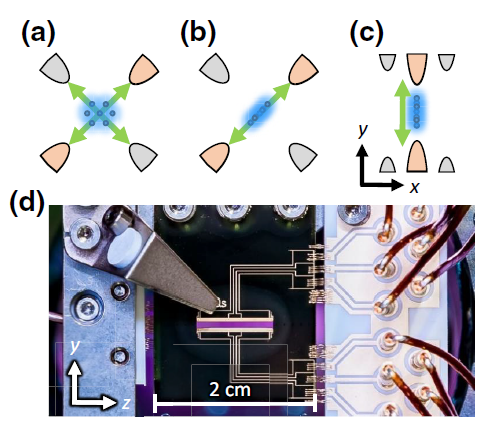
\includegraphics[width=\linewidth]{Kiesenhofer - Radial Trap.png}
    \caption{(\textbf{a}), (\textbf{b}) Radial cross section of a Paul trap. The RF and DC electrodes are represented in orange and gray repsectively. At the center of the electrodes is the ion crystal in blue. The green arrows represent the micromotions experienced by the ions. The ion crystal in (a) is oriented in the plane spanned by two radial direction. In (b) the crystal is oriented in the plane spanned by one radial direction and the axial direction. (\textbf{c}) This is a radial cross section of a three-layer trap. This configuration has the advantage of allowing optical access perpendicular to the micromotion. (\textbf{d}) A photograph of an ion trap in a vacuum chamber. The funnel aperture at the top left loads the ions from a calcium target. Figure borrowed and truncated from \textit{Controlling Two-Dimensional Coulomb Crystals of More Than 100 Ions In A Monolithic Radio-Frequency Trap}. Description is my own.}
    \label{fig:Radial Traps}
\end{figure} 

Neither orientation in Fig. \ref{fig:Radial Traps} has an advantage when it comes to RF-power requirements, however, the orientation in Fig. \ref{fig:Radial Traps}(b) only experiences driven micromotion along a single direction, which gives it an added benefit over the setup in Fig. \ref{fig:Radial Traps}(a). Building off of that, the three-layer trap in Fig. \ref{fig:Radial Traps}(c) maintains the beneficial crystal orientation while also giving optical access from directions perpendicular to the micromotion, allowing for laser cooling and laser addressing of individual ions. It's with this configuration that Kiesenhofer \textit{et al.} were able to demonstrate trapping of 2D crystals of over 100 ions \cite{Kiesenhofer}.

\subsubsection{Quantum Charge-Coupled Devices}
Among the variety of monolithic traps is a particular architecture known as a quantum charge-coupled device (QCCD). This is similar to the more common charge-coupled device (CCD) that's found in modern digital cameras. In the same way that a CCD stores imaging information as electrical charges that can be manipulated and moved around on the CCD, a quantum CCD contains separate regions that can hold and transport quantum information using dynamic electric fields \cite{Pino}. Each of these different regions on the QCCD performs one of various functions such as loading, interaction, and measurement. The advantage of doing things that way is that it becomes easier to optimize that aspect of the trap for it's singular function \cite{Bruzewicz}.

Scientists studying QCCD architecture have shown in small scale trapped-ion experiments that error rates can be kept low, and they're hopeful that similar results can be achieved when scaling. Pino \textit{et al.}, in 2021, introduced a scalable design for a cryogenic surface trap that integrates parallel interaction zones and fast ion transport into a QCCD foundation that could maintain the low error rates observed in individual ion crystals (see Fig. \ref{fig:QCCD}) \cite{Pino}.

QCCD architecture is promising, but it does face some challenges in creating a scalable quantum computer. Among other things, a succesful, scalable device, would need the ability to trap multiple small ion crystals, perform fast transport operations to move ions between crystals, and track qubit states across multiple zones. Each of those requirements can be met separately, but to combine those features into a single device presents a challenge. The device developed by Pino \textit{et al.} is capable of meeting all those requirements and more, however, they do not predict that it will scale to thousands of qubits or more. Their QCCD device could be scaled by placing multiple chip-traps end to end, however, that linear scaling would also linearly increase the transport time between connected circuits, putting a damper on sustainable coherence. A future approach might look at maintaining better connectivity through photonic interconnects (using flying qubits), possibly even leverage different types of connectivity at different scales \cite{Pino}.
\begin{figure}
    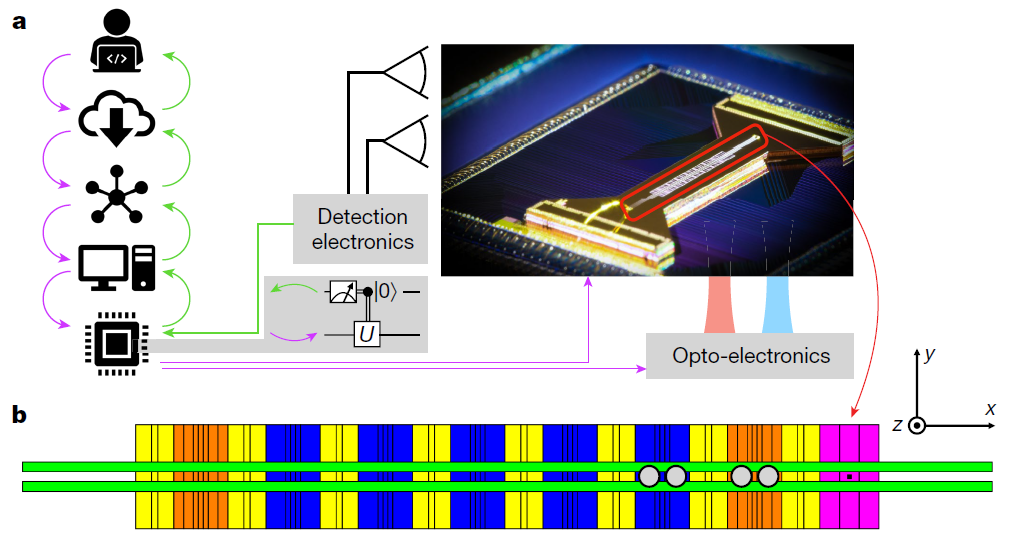
\includegraphics[width=\linewidth]{Pino - QCCD.png}
    \caption{(\textbf{a}) Left, a diagram of how information flows through the system: user, cloud, internal tasking, machine control, and field programmable gate array (FPGA). Right, a photopgrah of the QCCD trap. (\textbf{b}) Trap schematic. The long green wires are RF electrodes. Orange and blue are gate zones with yellow auxiliary zones in between. The gray circles indicate which gate zones were used in this work. Figured borrowed and truncated from \textit{Demonstration of the trapped-ion quantum CCD computer architecture}. Description is my own.}
    \label{fig:QCCD}
\end{figure}